\renewcommand{\theequation}{\theenumi}
\begin{enumerate}[label=\arabic*.,ref=\thesubsection.\theenumi]
\numberwithin{equation}{enumi}
\item No of bags having weight more than 5 Kg = 7
\\
total no of bags = 11
\begin{align}
P\left(A\right) &= \frac{7}{11}
\\
&=0.636
\end{align}
codes for the above equation can be get from here
\begin{lstlisting}
codes/prob/prob9.py
\end{lstlisting}
\begin{figure}[!ht]
	\centering
	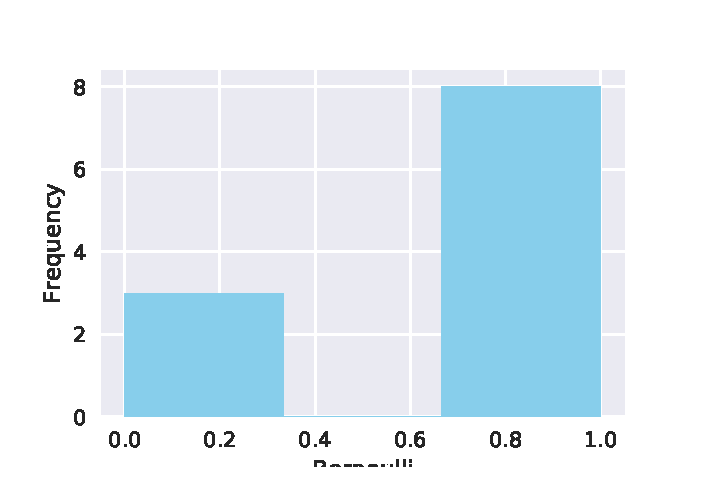
\includegraphics[width=\columnwidth]{./figures/prob/prob8.eps}
	\caption{probability of bag to be more than 5 Kg  }
	\label{fig:bt9}
	\begin{lstlisting}
	figs/prob/prob9.py
	\end{lstlisting}
\end{figure}
\end{enumerate}